\begin{sloppypar*}

    \begin{warning}
        \textbf{Disclaimer}: \textit{The following may not be accurate! Reader
        discretion is advised.}
    \end{warning}

    \noindent In order to compare the \textbf{modality choices} for the generation
    of functional embeddings for \textit{gene-products}, the authors have proceeded
    in two phases: \hfill\break
    \begin{tabularx}{\textwidth}{XX}
        1. prepare embeddings & 2. compare on downstream tasks
    \end{tabularx} \hfill\break
    In the first part various embeddings from different modalities are devised, 
    then, in the second part a comparison of these embeddings are performed on
    some benchmark downstream tasks.

    \subsection{Embedding preparations}
    \noindent Three embeddings' groups are devised, namely:

    \begin{tabularx}{\textwidth}{XXX}
        1. OMICS & 2. STRINGS & 3. PoPS
    \end{tabularx} \hfill\break
    \noindent For the \textbf{OMICS embeddings}, a Variational Deep Tensor Factorization
    Model is setup (Figure \ref{fig:omicsembed}), wherein, three data sources,
    namely, \textbf{DepMap}, \textbf{GTEx} and \textbf{ProtT5} are used. ProtT5
    \cite{protTrans} is a \textit{language-model}, that generates embeddings
    utilising protein sequences information from the previous two sources. So,
    the gene-sample matrices available from DepMap (essentiality screen) and
    GTEx (expression profile) are used directly for their part, and their processed
    version is output from ProtT5. The VDTF Model then attempts to learn gene
    embeddings and sample embeddings by reconstructing the three aforementioned
    matrices. A gradient reversal layer \cite{revGrad} ensures that the learnt
    gene embeddings ()$a_j$) are \textbf{unable} to distinguish between the three
    datasources, as part of bias mitigation scheme. \hfill\break

    \noindent The \textbf{STRING embeddings} were prepared in two versions, the
    first utilised the \textit{complete} gene-gene interaction graph and in the
    second the edges that were proven by manual curation were removed. On each
    GGI graphs, two algorithms were applied, \textit{viz.}, \textbf{node2vec}
    and \textbf{VERSE} and the resulting embeddings per gene were concatenated. \hfill\break

    \noindent For the \textbf{PoPS embeddings}, the \textit{polygenic priority score}
    features were downloaded as feature matrices, and two versions were created.
    In the first all info was retained, but, in the second, manually curated
    information was excluded. These feature matrices form the embeddings. \hfill\break

    \noindent The data sources are mentioned in detail in \textbf{Table 2} in the
    paper. The second versions for the STRING and PoPS embeddings are referred to
    as \textit{experimental}, and they aim at removing the street light effect.

    \begin{figure}
        \centering
        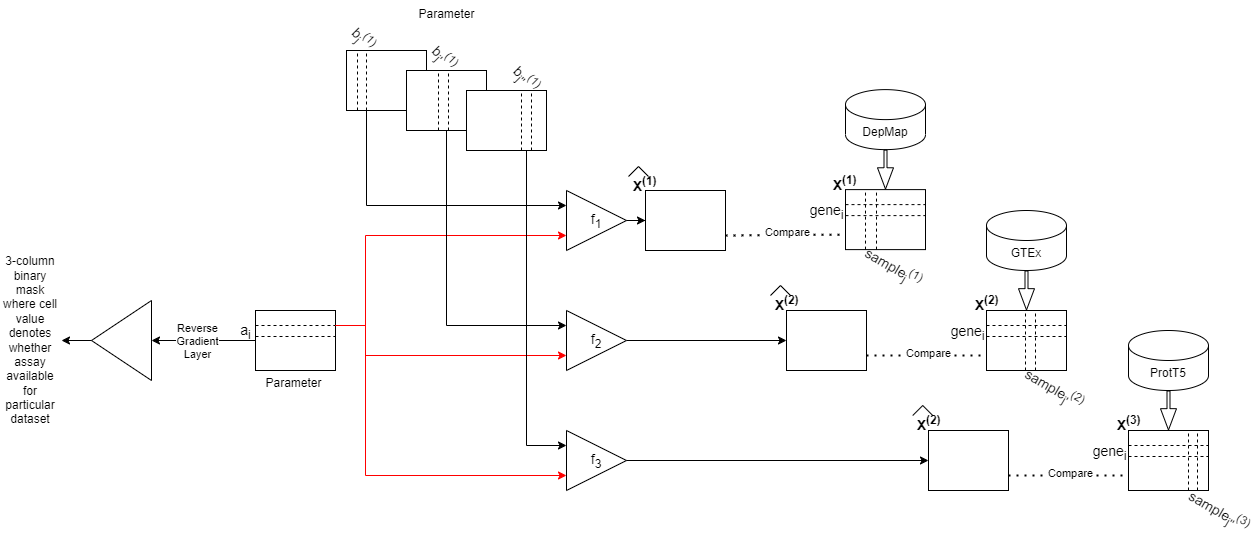
\includegraphics[scale=0.43]{omics.png}
        \caption{OMICS Embedding Generation}
        \label{fig:omicsembed}
    \end{figure}

    \subsection{Comparison on downstream tasks}
    A total of $6$ downstream tasks were setup, which can be grouped into three
    categories, namely, \textbf{human curated gene-lists/annotations} which had
    evidence in published literature, \textbf{statistical association scores},
    where the task was to predict the known scores and \textbf{annotation
    inequality assessment} which attempted to identify the bias. The performance
    of the embeddings are \textit{mixed} and the authors failed to conclude if
    one embedding was better than rest, in general.

    \subsubsection{Human curated}
    \textbf{1. Disease-Gene Prediction:} The dataset is obtained from $6$ sources
    mentioned in \textbf{Table 1} in the paper. XGBoost model is trained and
    tested for each embedding group, the task being, for all $6$ lists, whether
    or not a gene is part of it.

    \textbf{2. HPO Annotation Prediction:} The dataset is based on NCBI, Ensembl
    and STRING; the data and baseline results are obtained from HPOFiller (GCN)
    based. A $2$-layer multi-class classifier predicts the phenotype annotation
    for genes.

    \textbf{3. Cancer Gene Prediction:} The dataset is based on STRING and TCGA;
    the data and baseline results are obtained from EMOGI (GCN based). Again,
    XGBoost model was used to predict cancerous genes.

    \subsubsection{Association Studies}
    \textbf{4. Trait-Gene Association Prediction:} The data is obtained from UK
    Biobank's Genebass study and the target scores are computed using MAGMA. This
    task considered the rare variants. A logistic regression setup was used to
    match the MAGMA scores for traits per gene.

    \textbf{5. Gene level Association:} The data is obtained from UK
    Biobank's GWAS study for $22$ uncorrelated blood biomarkers and the target
    scores are computed using MAGMA. This task considered the common variants.
    The model was similar to that used in original PoPS study.

    \subsubsection{Annotation Inequality}
    \textbf{6. Publication-count Bin Prediction:} The publications' list for each
    gene covered in previous benchmarks was obtained from PubMed, and some method
    was used to classify each gene into a publication-count bin. The objective was
    to test if embeddings that did not have street light effect leaked into them
    could still predict counts reliably.
    
    % \begin{markdown}
    % \end{markdown}
    % \begin{figure}
    %     \centering
    %     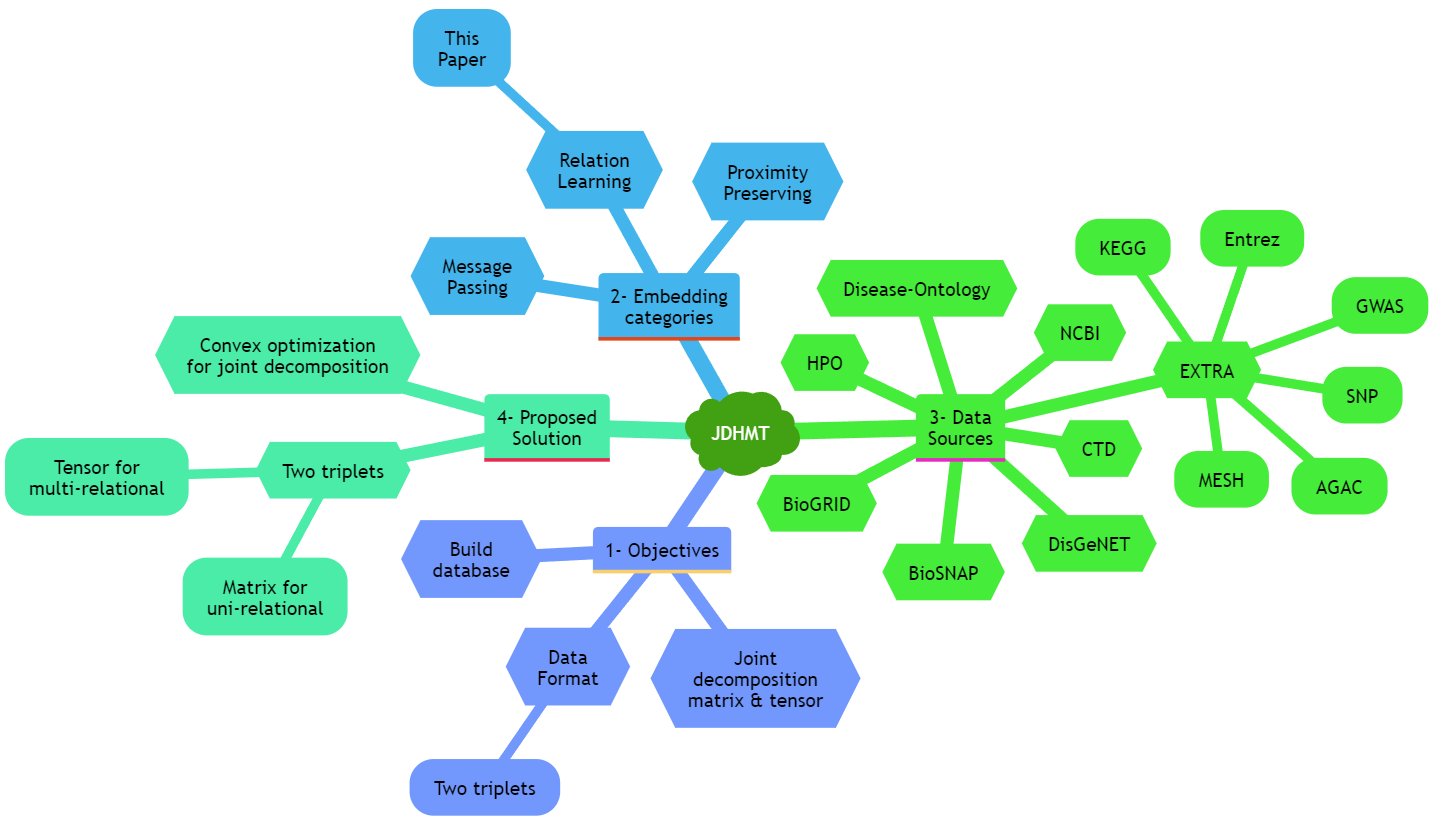
\includegraphics[width=170mm,scale=1]{mindmap.png}
    %     \caption{Mindmap}
    %     \label{fig:mindmap}
    % \end{figure}

    % \begin{mybox}
    %     Since my study pertains to understanding the embedding generation, the
    %     intrinsic and extrinsic evaluations are not discussed.
    % \end{mybox}
    
\end{sloppypar*}